\chapter{User Story Mapping}

El mapa de historias de usuarios es una forma muy visual de organizar las historias de usuario y sus tareas relacionadas.

\begin{figure}[h]
    \centering
    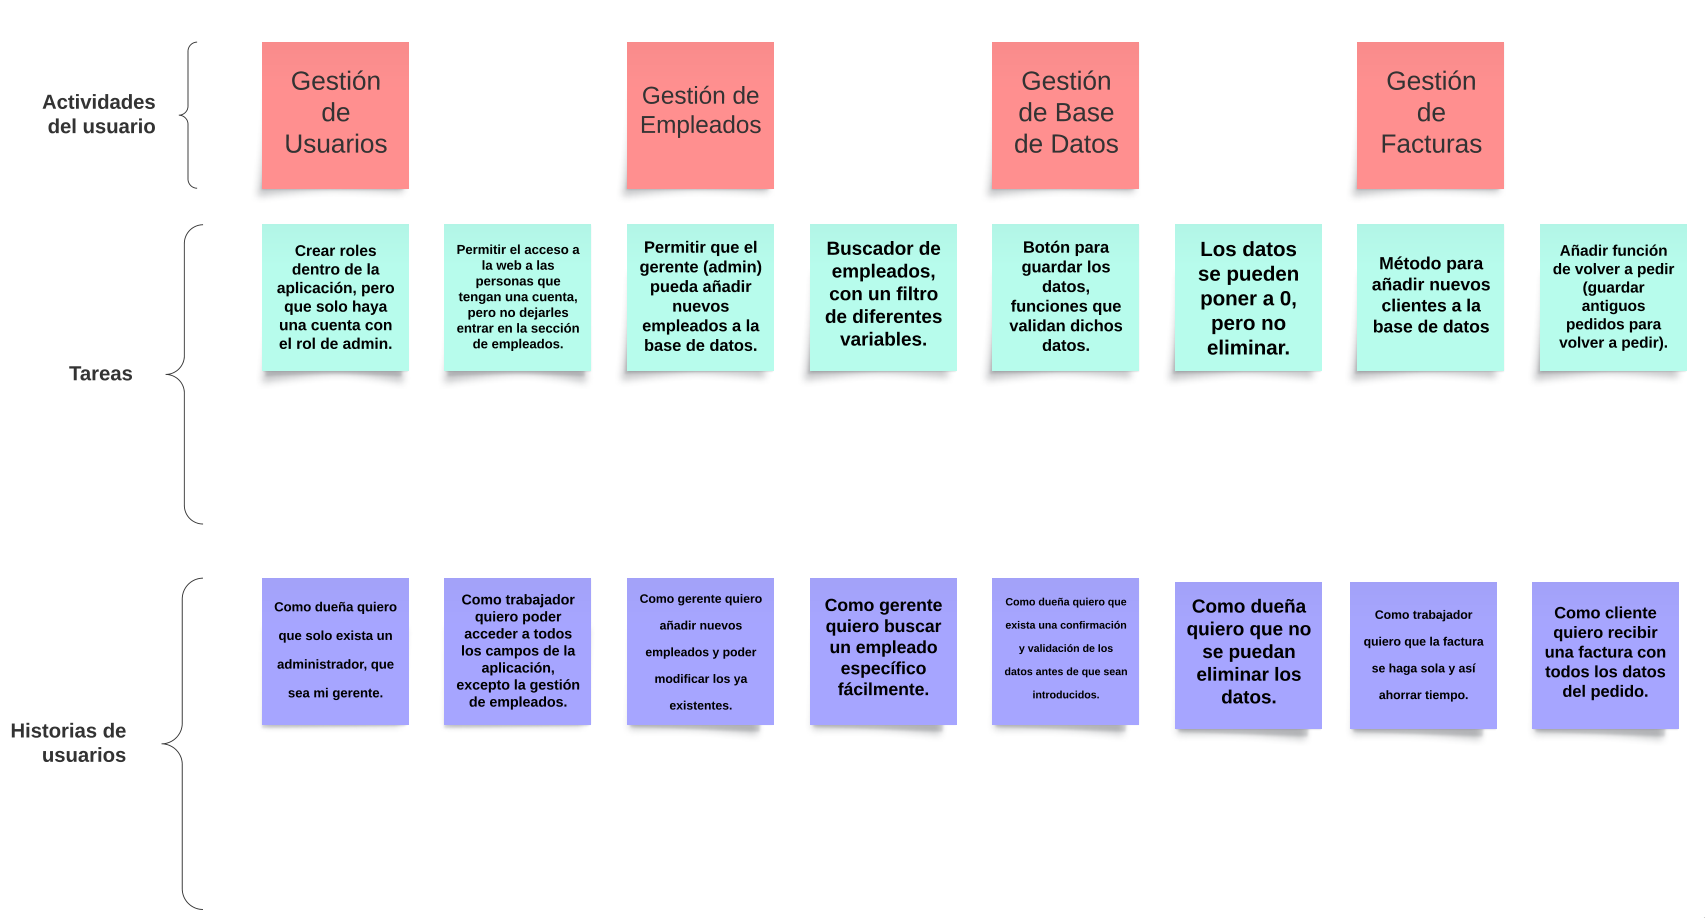
\includegraphics[width=1\textwidth]{figures/mapa-historias-usuarios-1.png}
    \caption{Pimera parte del mapa de las historias de usuario}
    \label{fig:user-story-mapping-1}
\end{figure}

\begin{figure}[h]
    \centering
    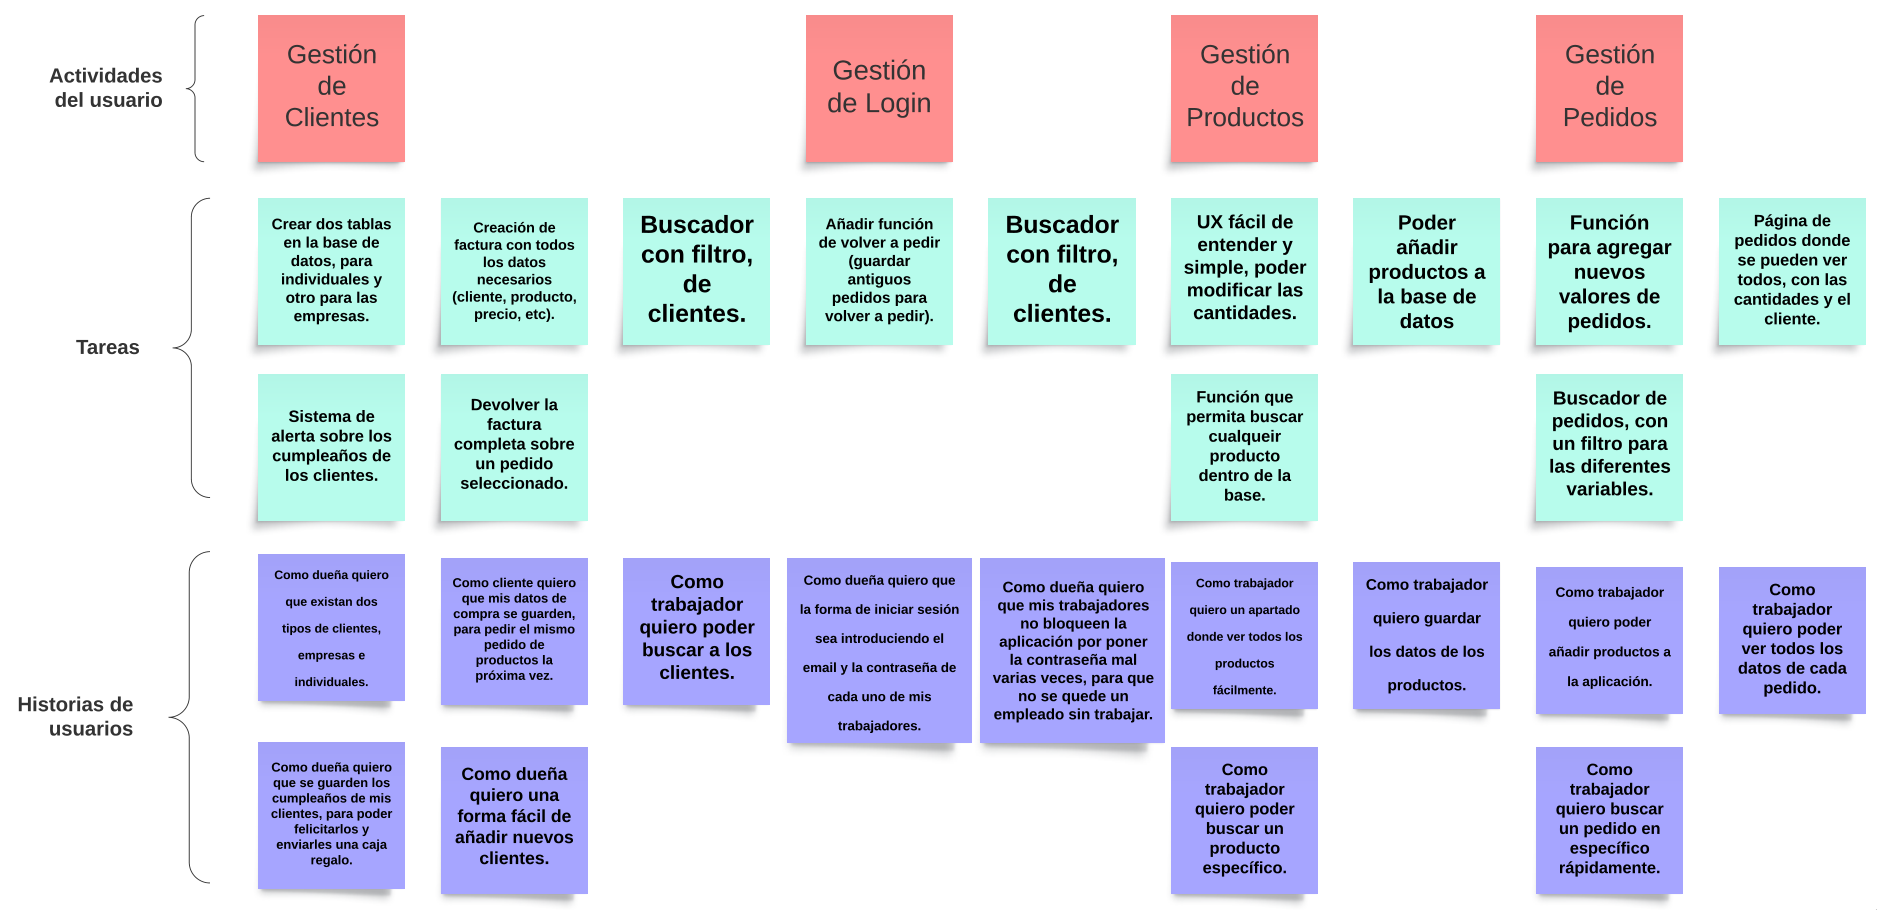
\includegraphics[width=1\textwidth]{figures/mapa-historias-usuarios-2.png}
    \caption{Segunda parte del mapa de las historias de usuario}
    \label{fig:user-story-mapping-2}
\end{figure}
